\chapter{Synthesis of Decoupled Computational Pipeline on FPGAs}
\label{decoupleChap}
As mentioned in~\ref{chap1:hls}, the HLS tools statically schedule
operations when generating accelerators, whose runtime behavior
is therefore rather simple. Different parts
of the generated circuit run in lockstep with each other, no dynamic dependency checking mechanisms,
such as scoreboarding or load-store queueing, are needed.
This rigid scheduling of operators, while producing hardware of simpler structure and smaller area,
is also vulnerable to stalls introduced by cache misses or variable latency operations.
\begin{comment}
It is a common design practice to have data explicitly moved in and out of chip through
instantiation of DMA engines~\cite{vivado_hls:appnoteMMult}, and coordinate the computation with transfer of data
through using software. There are also tools~\cite{coram} which hide the 
complexity of managing memory
hierarchy from the user by providing a standard abstraction
of data access interfaces. The FPGA designers can use the
provided primitives to explicitly manage data movement between
the on-board memory and the SRAM on-chip, allowing
locally-addressed memory access by the computation pipeline.
A set of regular kernels are synthesized to this architecture
in~\cite{c2coram}, demonstrating its applicability in the context of high level
synthesis.
\end{comment}
In this chapter, we present a flow which alleviates this problem by structuring the
computations and data accesses in the original program into a series of coarse-grained pipeline stages, through which data can stream through. This pattern takes advantage
of the FPGAs being throughput-oriented devices, while naturally overlaps computation and
communication in the applications.


\begin{figure}[htp]
\begin{center}
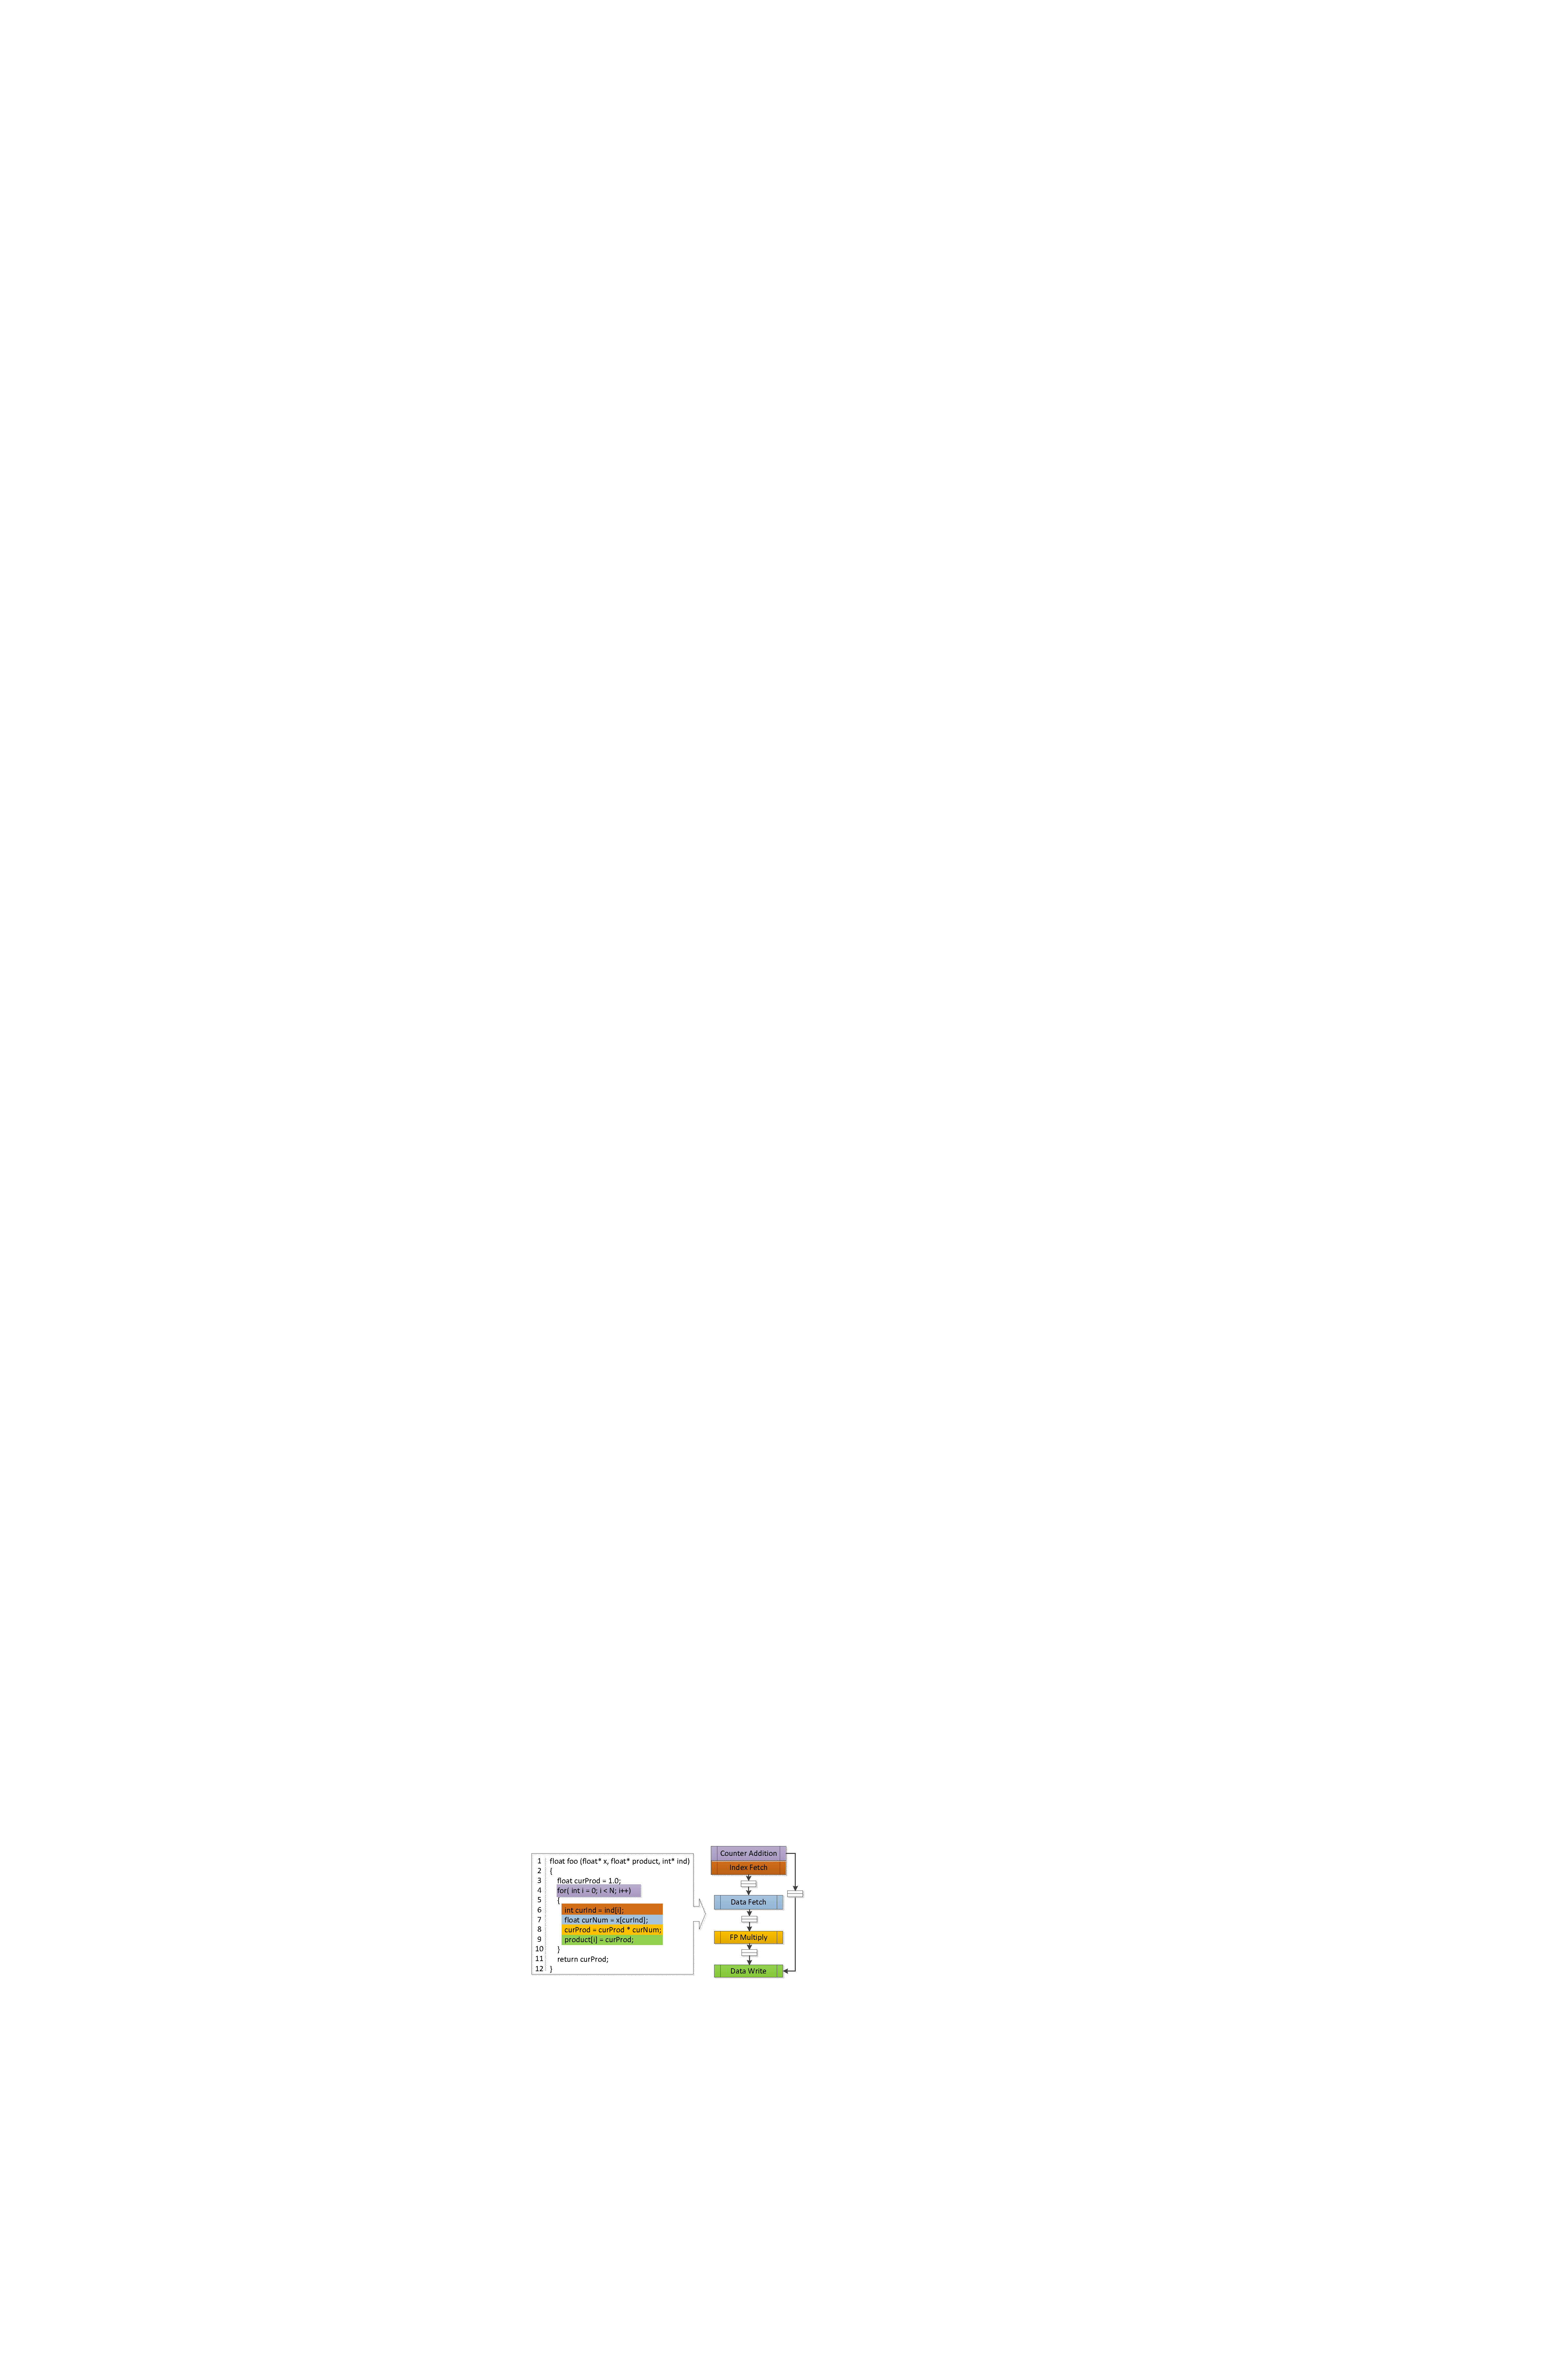
\includegraphics[width=0.6\linewidth]{chap3fig/motExample.pdf}
\caption{Converting a Simple Function to Decoupled Computational Pipeline
\label{fig:motivating}}
\end{center}
\end{figure}

\section{A Motivating Example}
\label{motex}
Shown in figure~\ref{fig:motivating} is a simple example where separating a software kernel into multiple decoupled stages can improve the overall performance. As the shown function
is pushed through the conventional HLS flow, opportunities for parallelization are
discovered and a static schedule can be generated. The loop counter addition and the loading of $curInd$ can happen simultaneously, and the next iteration of the  loop
can start before the current iteration finishes. Meanwhile, because the floating-point
multiply always uses its result from the previous iteration, the shortest interval with which we can start a new iteration is limited by the latency
of the multiplier. The execution schedule of this function is shown in figure~\ref{fig:sche}(a).

This execution schedule, unfortunately, assumes the best case latency for all the memory accesses. Since the computation kernel is turned into a monolithic accelerator,
the centralized controller would have to stall the entire compute engine when long latency off-chip communication operations are occurring. This is less of an issue when the memory access patterns are known \textit{a priori}, such that the data can be moved on-chip before
it is needed, or if the data set is small enough to be entirely buffered on the FPGA.
However, in this example, just like in many interesting algorithms, the data access depends on the result of computation and the memory footprint requires the use of off-chip storage. Figure~\ref{fig:sche}(b) shows the execution of the generated hardware module
in the presence of cache miss stalls. Note how the slowdown reflects the combination
of all cache miss latencies. This does not have to be the case though, since there are
parts of the computation graph whose progress does not need the memory data to be immediately available. These sections should be able to move forward. This extra bit of
freedom in the execution schedule can potentially have a significant effect.

In this example, it is possible to decouple the execution of the floating point multiply and the data accesses from each other. Without a unified schedule, one load operator can keep requesting new data while the other one waits for previous requests to be responded by off-chip storage, and the floating point multiplier works through
previously fetched data. This is achieved by having one module responsible for each
of the memory accesses and the multiplication, as shown in figure~\ref{fig:motivating}.
The FIFOs allow for the communication between these modules, while buffering the data
already produced but not yet consumed. Over a long period of time, the stalls introduced by the memory accesses are shadowed by the long latency of the floating point multiplier, who is always supplied with the backlog of data in the FIFO when
cache misses occur. As long as the overall bandwidth provided by the memory subsystem
satisfies the need of the computation, the latency of the memory accesses can be
tolerated. 

Figure~\ref{fig:sche}(c) shows the execution schedule when the decoupled pipeline is used. The latencies through the FIFOs are not taken into consideration here, e.g. FP multiply starts immediately after completion of $curNum$ load, but their effect
should be minimal when amortized over a large number of iterations. 


\begin{figure}[htp]
\begin{center}
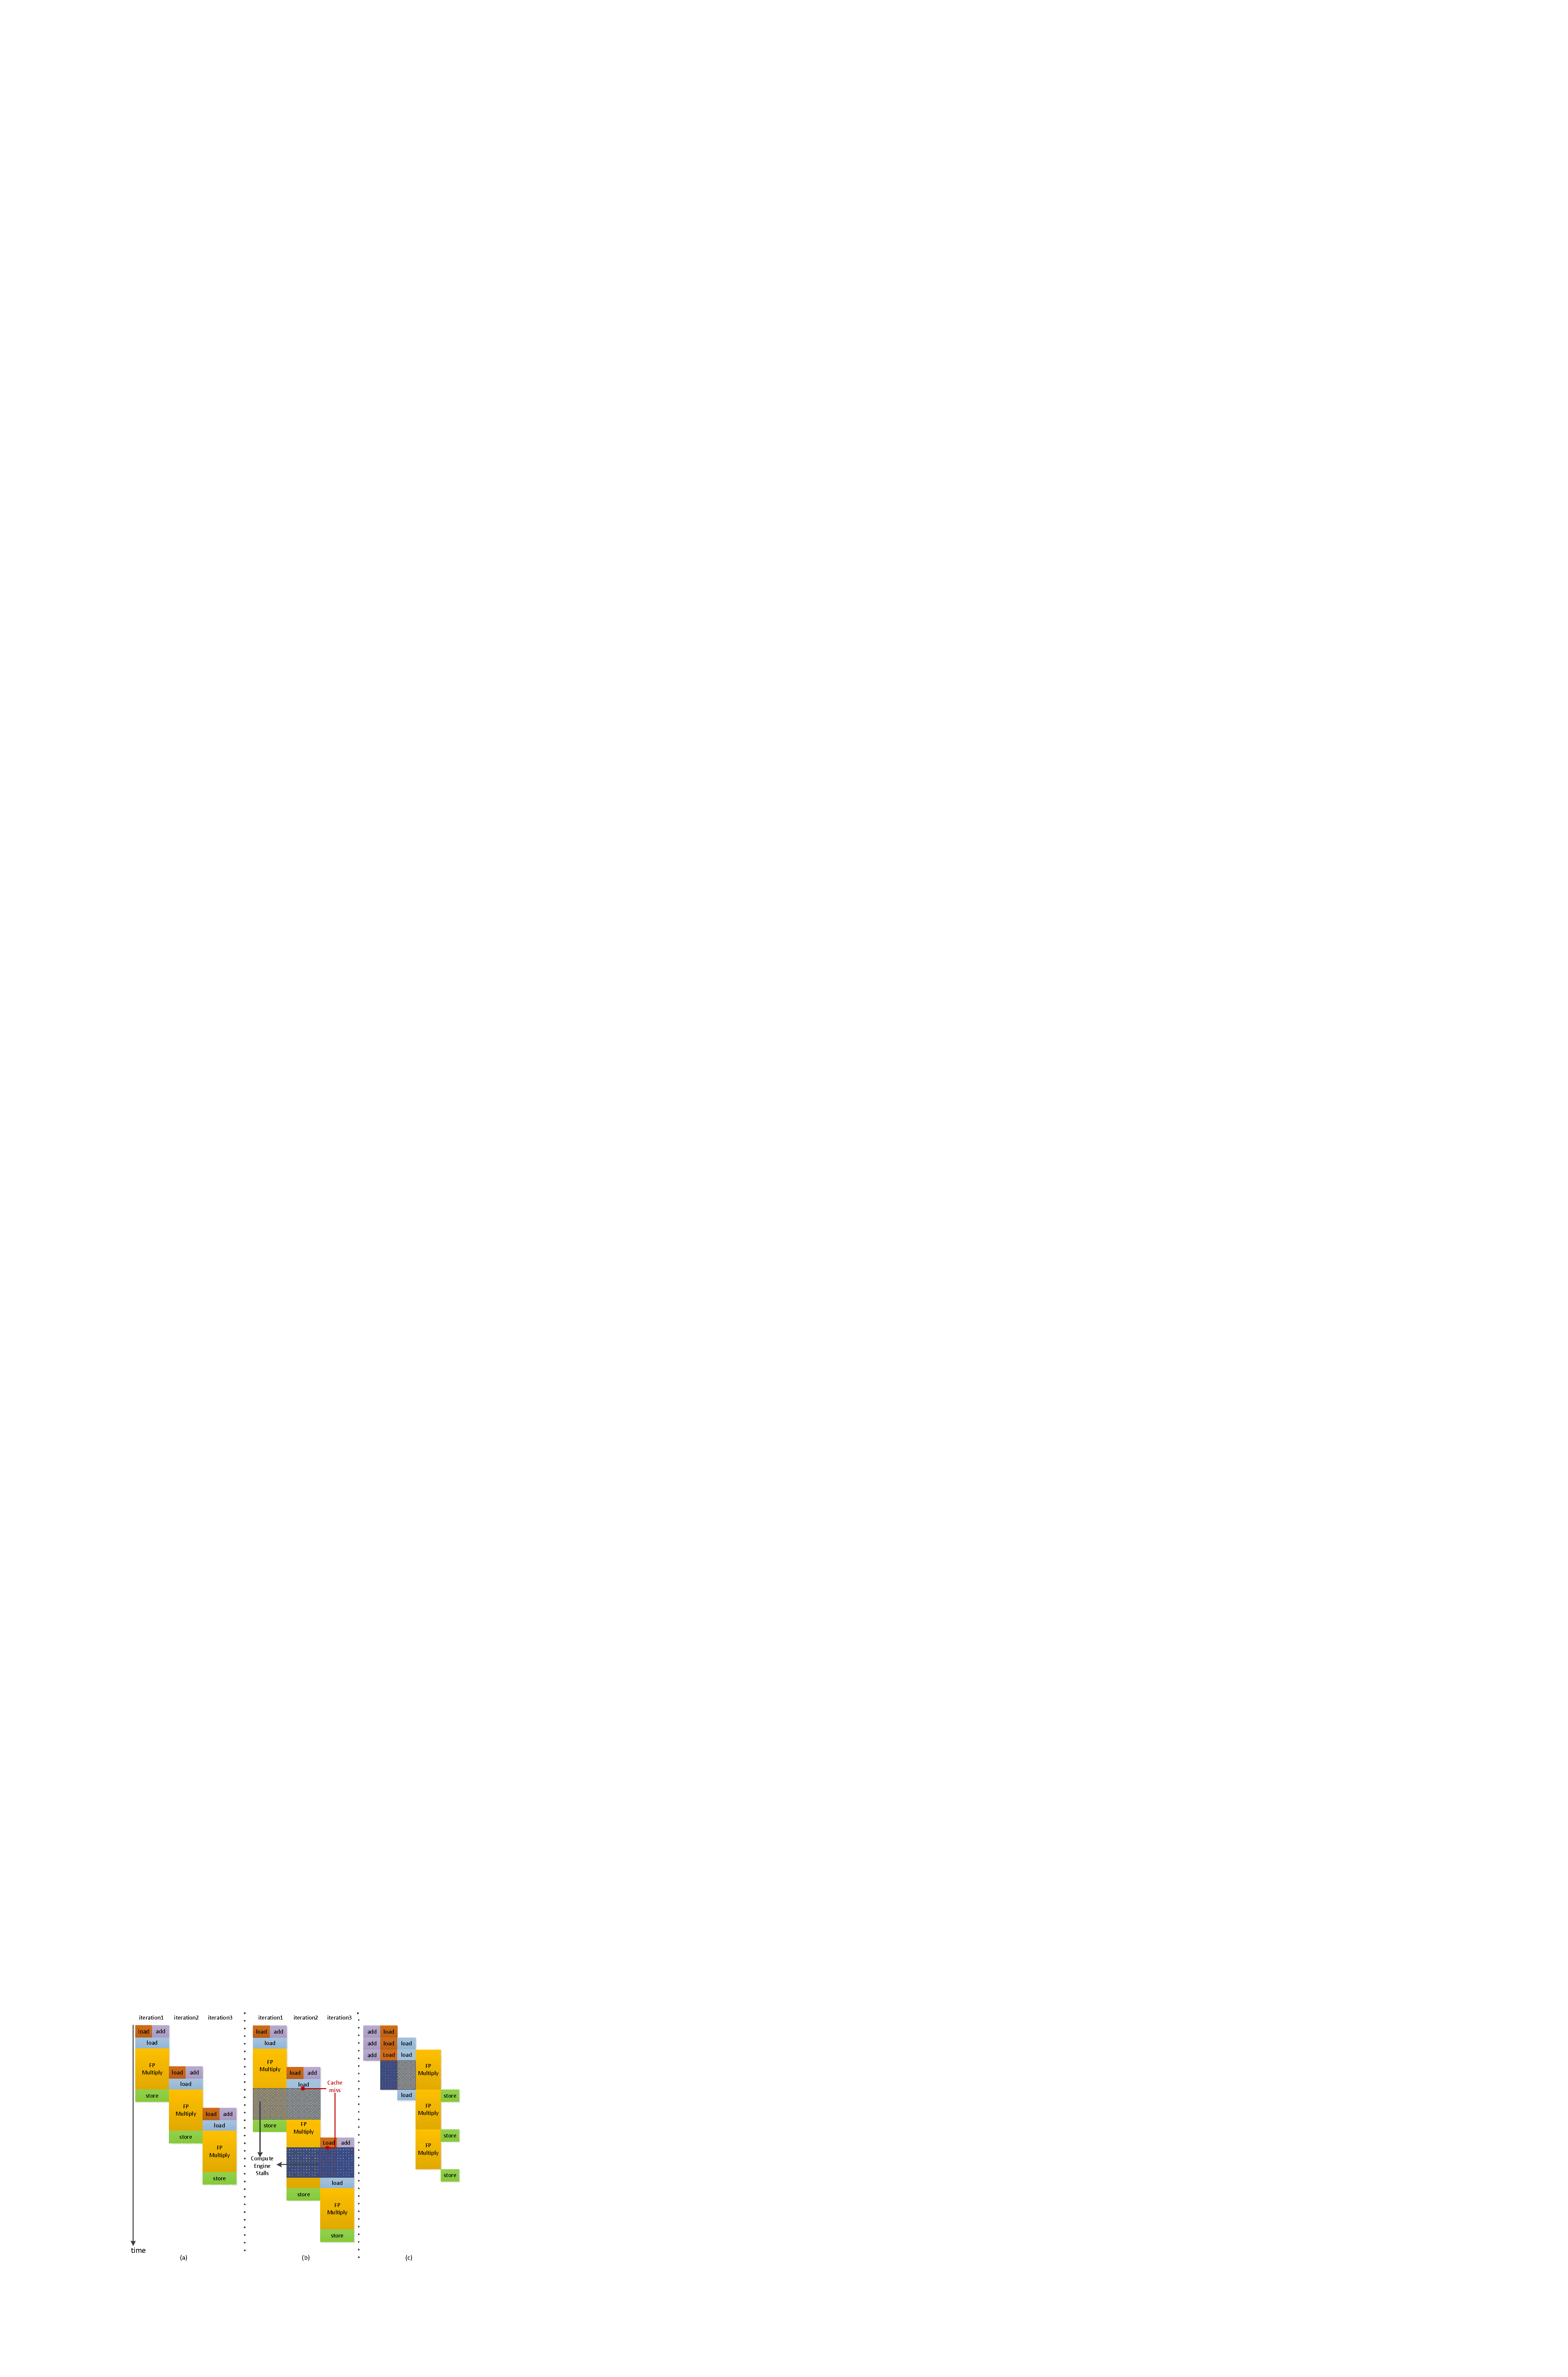
\includegraphics[width=1.0\linewidth]{chap3fig/schedules.pdf}
\caption{(a) Static schedule produced by HLS (b) Actual Execution with Cache Misses (c) Execution of Decoupled Computational Pipeline 
\label{fig:sche}}
\end{center}
\end{figure}

\section{Partitioning the Instructions}
\label{sec:partins}
To generate modules who are running out of sync from each other, the original
control data flow graph (CDFG) needs to be partitioned into multiple sets.
Each set is to be converted to a self-contained function and synthesized to
a stage in our pipeline.
To maximize the performance of the resulted implementation, a few factors
should be considered during our partitioning process. 
First, circular dependencies between
nodes of the innermost loop need to be contained within each set. These strongly
connected components (SCCs) in CDFG are associated with
loop carried dependencies, and are the limiting factors for how
aggressively loop iterations can be overlapped. The initiation
interval (II) of loops are dictated by the latency of these cycles.
As the communication channels will always add latency,
having parts of an SCC in CDFG scattered across multiple
stages would increase the II of the iterations, which are now
executed in a distributed manner. 
Secondly, as we have demonstrated in section~\ref{motex}, with memory operations separated
from dependency cycles involving long latency compute, we
can have cache misses completely hidden by the slow rate
of data consumption.
Thirdly, to
localize the effects of stalls introduced by cache misses, the
number of memory operations in each set should be
minimized, especially when they address different parts of the
memory space.



 


%\begin{figure}[htp]
%\begin{center}
\begin{algorithm}[t]
  \caption{Instruction Partitioning}\label{algo1}
  \begin{algorithmic}[1]
  \Procedure{PartitionCDFG}{G}%\Comment{G: CDFG of loop nests}
    \LineComment{SCCs of instructions formed with data/control/memory dependency edges}
    \State SCCs $\gets$ allStronglyConnComps(G)
  \State DAG $\gets$ collapse(SCCs,G)
  \State topoSortedNodes $\gets$ topologicalSort(DAG)
  \State longSCCs $\gets$ getSCCWithLongOp(SCCs)
  \State memNodes $\gets$ findLdStNodes(G)
  \State memLongSCC $\gets$ LongSCCs $\cup$ memNodes
  \State allSets $\gets \{\}$
  \State curSet $\gets \{\}$
  \While{topoSortedNodes $\ne \emptyset$}
     \State curNode $\gets$ topoSortedNodes.pop()
     \State curSet $\gets$ curSet $\cup$ curNode
    
     \If{curNode $\in$ MemLongSCC}
     %\If{$curSubG \cap MemLongSCC \ne \emptyset$}
    \State allSets $\gets$ allSets $\cup$ curSet
    \State curSet $\gets$ \{\}
     %\EndIf
     \EndIf

     %\State $curSubG \gets curSubG \cup curNode$
     
  \EndWhile
  \State \Return allSets 
  %\State $OtherNodes = G - SCCs - MemNodes$
  %\State $SNodes\gets collapseSCC(G, SCCs)$
    %\State $i\gets 0$
    %\foreach{$r\not=0$}\Comment{We have the answer if r is 0}
  %\State $SGs\gets ClusterWithSeed(SCCs, MemNodes)$
  %\State $MGs\gets ClusterWithSeed(MemNodes, MemLongSCC)$
  %\State $OGs\gets ClusterWithSeed(OtherNodes, MemLongSCC)$
  %\State \Return $SGs \cup MGs \cup OGs$
  %\While{$SCCs \ne \emptyset$}
  %  \State $curSubG\gets \{\}$
  %  \State $curSCC\gets SCCs.pop()$
  %  \State $DFSCluster(curSCC,curSubG,MemNodes)$
  %  \State $Subgraphs\gets Subgraphs \cup curSubG$
  %\EndWhile
  %\While{$MemNodes \ne \emptyset$}
  %  \State $curSubG\gets \{\}$
  %  \State $curMem\gets MemNodes.pop()$
  %  \State $MemLongSCC\gets LongSCCs \cup MemNodes$
    %  \State $DFSCluster(curMem,curSubG, MemLongSCC)$
  %  \State $Subgraphs\gets Subgraphs \cup curSubG$
  %\EndWhile
  %\While{$OtherNodes \ne \emptyset$}
  %  \State $curSubG\gets \{\}$
  %  \State $curN\gets OtherNodes.pop()$
  %  \State $MemLongSCC\gets LongSCCs \cup MemNodes$
    %  \State $DFSCluster(curN,curSubG, MemLongSCC)$
  %  \State $Subgraphs\gets Subgraphs \cup curSubG$
  %\EndWhile
  %now do the otherNodes
  
    %\EndWhile\label{euclidendwhile}
    \EndProcedure
  %\Procedure{ClusterWithSeed} {$seeds$, $excludeSet$}
  %\State $subgraphs\gets \{\}$
  %\While{$seeds \ne \emptyset$}
    %\State $curSubG\gets \{\}$
    %\State $curN\gets seeds.pop()$
    %\State $DFSCluster(curN,curSubG, excludeSet)$
    %\State $subgraphs\gets subgraphs \cup curSubG$
  %\EndWhile
  
  %\State \Return $subgraphs$
  %\EndProcedure
  
  %\Procedure{DFSCluster} {$curN$, $curG$, $excludeSet$}
  %\If{$curN.isCovered()$}
  % \Return
  %\EndIf
  
  %\If{$curN \in excludeSet$}
  % \If{$curG \cap excludeSet \ne \emptyset$}
  %   \Return
  % \EndIf
  %\EndIf
  %\State $curG \gets curG \cup curN$
  %\State $curN.setCovered(true)$
  %\State $nextNodes\gets getDependents(curNode, DAG)$
  %\While{$nextNodes \ne \emptyset$}
  % \State $nextNode \gets nextNodes.pop()$
  % \State $DFSCluster(nextNode, curG, excludeSet)$
  %\EndWhile
  %\EndProcedure
  \end{algorithmic}
\end{algorithm}

\subsection{Partitioning Algorithm}
The first factor was one of the observations made 
in~\cite{dswp}, where sequential programs were converted into multithreaded
codes running on multicore processors. Their algorithm
finds strongly connected components (SCCs) in the
original dataflow graph, collapses them into nodes and then
heuristically partitions the resulted directed acyclic graph
(DAG) into threads with balanced load. In our flow, the search
for SCCs is also necessary and its outcome is used for the
ensuing partitioning, which centers upon memory operations.
In Algorithm~\ref{algo1}, the steps taken to perform the partitioning are detailed.
The SCCs are collapsed into new nodes, which together with the original nodes in the CDFG, are topologically
sorted. The obtained directed acyclic graph is traversed and a new set is created whenever a memory operation
or an SCC with long latency computation
is encountered. Here, long latency operations are those which cannot be completed within
one clock cycle, and
their categorization ultimately depends on the target frequency
of the final implementation on the FPGA. Currently, we
leverage Xilinx’s Vivado HLS to generate latency estimate for
various compute operations. With a target clock frequency of
150MHz, for instance, floating point multiply takes four clock
cycles while a 32 bit integer addition can be completed within
a cycle. As Vivado HLS is eventually used as the backend for
our HDL generation, it provides accurate annotations for our
flow.
\begin{figure}[htp]
\begin{center}
\includegraphics[width=0.9\linewidth]{chap3fig/order.pdf}
\caption{Three Types of Memory Dependencies
\label{fig:memorder}}
\end{center}
\end{figure}
 
\subsection{Preserving Memory Dependency }
\label{subsec:pmd}
The semantics of the input high level language often create
dependencies implicitly carried by memory accesses.
Given two statements in a program, Bernstein's conditions~\cite{4038883} described when
they are independent and can be executed in parallel or out of order.
If two memory operations access the same location and one of them is a store, their order in the original program execution must be preserved. More specifically, three types of dependencies need to be observed:
\begin{itemize}
    \item Read-after-write (RAW) -- When the same memory location is written by one statement and read by the other, there is a dataflow dependence between them (figure~\ref{fig:memorder}a). Performing them out of order results in the outdated operand to be used by the consumer statement. 
    
    \item Write-after-read (WAR) -- When a memory location is read by the first statement and subsequently written by the second, there is an anti-dependence between them (figure~\ref{fig:memorder}b). Performing them out of order overwrites
    the correct operand prematurely. 
    \item Write-after-write (WAW) -- When both statements write to the same location, there is an output dependence between them (figure~\ref{fig:memorder}c). Reordering the two
    writes exposes the wrong value to the subsequent reads.
\end{itemize}
 For every pair of operations whose ordering needs to be preserved, a special dependency edge is added between them. Since the generation of the sets is performed around strongly connected components in the original dataflow, it is important to avoid adding unnecessary memory dependency edges. To achieve this, our flow currently relies on alias analysis to perform partitioning of the memory space. Accesses to disjoint memory regions can be safely reordered. When the source code contains pointer arithmetic or irregular memory accesses, compile time alias analysis may produce overly conservative results, in which case user annotations can be used to provide hints to the tool, similar to~\cite{manycache}. This partitioning of memory space naturally leads to creation of multiple data access interfaces, whose interactions with the memory subsystem can be customized, as will be elaborated in section~\ref{sec:optmem}.  



Under certain circumstances, we do not want to directly add edges between memory operations
as they hinder the CDFG partitioning. For the example in figure~\ref{fig:barrier}, during the execution of one outer loop iteration, the set of memory addresses accessed by the the load does not intersect
with that of the store instruction. However, across different outer loop iterations, these
two instructions can accesses the same locations. 
We can conservatively make them dependent
on each other, but this creates an SCC that ultimately prevents any partitioning, as can be
seen in the figure.



%become the performance bottleneck. 
Alternatively, a memory barrier can be inserted after the completion of 
each outer loop iteration. To implement the barrier in the pipeline, the stage containing
the semantically earlier instruction sends tokens to stages who contain the successor
instructions. Eventually during the RTL generation, the local schedule of instructions also needs to be constrained such that the sender of the barrier tokens is not reordered to before its predecessors, while the receivers execute before its semantic successors as well.

The insertion of the sender/receiver of the barrier happens after the instruction partitioning. Depending on if a partition is the sender or receiver of the token,
an extra store/load operation is introduced into the set of instructions, associated
with the basic block where the barrier occurs.

\begin{figure}[htp]
\begin{center}
\includegraphics[width=1.0\linewidth]{chap3fig/barrier.pdf}
\caption{Barrier for Enforcing Order of Memory Accesses
\label{fig:barrier}}
\end{center}
\end{figure}

\subsection{Control Dependency Edges}
Another source of edges in our CDFG -- control dependency, also warrants some 
discussion. The simplest way to add the control dependency edges is to have
every instruction dependent on the control transfer instructions of the immediate
predecessors of its container basic blocks. For a loop nest, this will necessarily
create a single SCC with all the branch instructions of the basic blocks within the loop nest. Essentially, a control flow ``backbone" is generated and the branch
tag tokens will need to be sent to all other modules whose instructions are predicated on these branches. The pipeline thus generated, while valid, may
have higher communication channel count and less opportunities for optimization
within each module, which will be elaborated more in section~\ref{sscf}. We thus
perform a more aggressive predication/control edge insertion by looking for the
earliest branch outcome which necessarily leads to the execution of an instruction. Given an instruction $i$ and its container basic block $bb$, our
flow looks for the nearest set of basic blocks $BB'$ who are not properly post-dominated by $bb$,
and insert the dependency edge between the branch instructions ending each member of $BB'$ and $i$.




\begin{comment}
Also, to ensure the barrier tokens are sent out only after the completion of preceding 
memory operations, which are often signaled by special \textit{RESP} lines,  a special module is created to monitor and coordinate the transmission of the tokens. Its structure
is shown~\ref{}, only when 
As we are trying to ensure the semantically later instructions
do not get ahead of their predecessors, the barrier is implemented by having the stage containing the later instruction sending tokens to an earlier stage in the pipeline. As the local schedule 
\end{comment}

%There is a possibility that the load instruction of an later outer loop iteration occurring 

%in the inner most loop can be separated as the memory dependency edges do not form a circle. However, 


\section{Construction of Pipeline of Subgraphs}
\label{sec:consp}


With instructions partitioned into disjoint sets, the flow then
reconstruct subgraphs from these sets of instructions. Each subgraph
contains a subset of the original control flow/basic blocks and 
will later be synthesized as a self-contained function. The reconstruction process involves adding relevant basic blocks according to the
association of the instructions with the current set.
\begin{itemize}
    \item For every instruction $i$  in the current set, recreate
    its container basic block if it's not already in the current subgraph.
    \item For every instruction $j$  $i$ depends on, 
    recreate its container basic block if it's not already
    in the current subgraph.
    \item If $j$ is associated with another subgraph, a load operation
    is created locally as a placeholder in its container basic block.
    \item If $i$ is producing operands for instructions assigned to 
    other sets, a store operation is inserted after $i$.
\end{itemize}
The set of recreated basic blocks $B$ are thus associated with either the instructions
assigned to the subgraph, or the placeholder instruction supplying them with operands. To mirror the relevant execution path in the original program, a few more steps need to be taken.
\begin{itemize}
    \item In the control flow of the original program, find the nearest common dominator $d$ of all the recreated basic blocks $B$, and add $d$ to $B$. It will be the entry block of our
    control flow in this subgraph.
    
    \item Find all the paths $P$ from $d$ to $b \in B$, add all the 
    basic blocks in each $p \in P$ to $B$.
    \item From each $b \in B$, find the paths $P_b$ to every $b' \in B$ without passing through $d$. Add all the basic blocks in each $p_b \in P_b$ to $B$. \item Create the branching instructions at the end of each $b \in B$. If the branching instruction was already assigned to the current subgraph, nothing needs to be done, otherwise a load operation is created to accept
    a branch target token from another subgraph, and then the actual branching is performed according to the received token. 
    \item If $d$ was inside a loop in the original control flow, any branch out of the set $B$ is redirected to $d$. Otherwise, any branch out of the set $B$ terminates the execution of this subgraph.
\end{itemize}


\begin{figure}[htp]
\begin{center}
\includegraphics[width=1.0\linewidth]{chap3fig/totalflow.pdf}
\caption{(a) The Motivating Example in Single Static Assignment Form (b) Partitioning of Instructions (c) Pipeline of Reconstructed Subgraphs
\label{fig:totalFlow}}
\end{center}
\end{figure}

In the control flow graph of the original program, the set of paths whose starting points and end points both fall in $B$ can be divided into
two groups. Some of these paths never reach basic blocks outside of $B$, and the rest go out of $B$ and then come back into $B$ via $d$. 
The first group
is completely contained within our subgraph.  If there is any path in the second group, then $d$ must be inside a loop, in which case we have effectively enclose the subgraph with a \textit{while(true)} loop and the execution of the part
of the path within the subgraph
will be repetitively activated by the availability of the proper tokens.

The insertion of load and store operations is necessitated by various
dependencies between the generated subgraphs. Other than data and control (branch) tokens we have mentioned, special tokens are also sent when ordering
of memory accesses needs to be enforced. Each of the inserted operations corresponds to a hardware queue between the decoupled modules, the flow of
tokens ensures the execution path are synchronized across different subgraphs
and the right operands are supplied for computations distributed across the
pipeline.
\begin{comment}
The dependencies between the generated subgraphs necessitate the insertion of communication primitives. In our case, these correspond to the load and store operations to/from a hardware queue between the decoupled modules.  
Other than the explicit data flows, control dependencies are also communicated using branch target tags, such that the local branch operations can synchronize across different subgraphs. Lastly, in the case where ordering of memory accesses needs to be enforced, special tokens are sent between modules.
\end{comment}
Eventually, in the hardware module synthesized from each subgraph, these loads and stores are blocking, as they operate on standard FIFO interfaces. Flow control between different pipeline stages are thus naturally introduced. 



The implementation of our partitioning algorithm and the insertion of the communication primitives leverage the LLVM infrastructure~\cite{llvmflow}. The LLVM front end converts the instructions in the original program to the single static assignment (SSA) form, which makes it easy to track dependencies and thus facilitates all the steps in our algorithm.
In figure~\ref{fig:totalFlow}, the conversion process from the example function (in SSA form) to the final pipeline of subgraphs is illustrated. For better readability, we have converted the LLVM intermediate representation to a less verbose, C-like version. Operators not available in C are explained in the figure.
To highlight
the inserted communication primitives, we show them as ``push" and ``pop" function calls taking in the queue name and the data vairable name as the parameters. The execution of the entire processing pipeline is completed when all modules are idling waiting for inputs and all hardware queues are empty. The runtime behavior of this pipeline thus resembles a streaming processing engine, with uncertainties introduced by memory access nodes smoothed out by FIFOs.
%As shown in figure 2, subgraphs whose first instruction reads value off a FIFO should be placed in an infinite loop to ensure it is repeated the right number of times, which is especially important if the subgraph is strictly within a loop. The execution of the entire processing pipeline is completed when all modules are idling waiting for inputs and all hardware queues are empty. The runtime behavior of this pipeline thus resembles a streaming processing engine, with uncertainties introduced by memory access nodes smoothed out by FIFOs.

% Figure 2 illustrates the result of clustering on our earlier example. Each of the generated subgraphs (SGs) corresponds to a decoupled stage in figure 1. For better readability, we have converted the LLVM intermediate representation to a less verbose, C-like version. Operators not available in C are explained in the figure.
%After the partitioning, the edges spanning two stages will be converted to communication channels 
%for data/control tokens 
%to be passed between them. From each stage's perspective, these are just normal load/store operations
%from/to special pointers corresponding to communication interfaces. During the actual hardware
%generation, FIFOs will be instantiated and connected. 




\begin{comment}
Conceptually, a
topological sort is performed on the DAG formed after the
SCCs are collapsed into single nodes. In the linear array thus
obtained, we find memory operations and SCCs with long
latency compute operations, which are tagged as “terminals”
for our clustering process. The algorithm then traverses the
array, starting a new cluster every time a “terminal” is added.
The detailed steps involved are shown in Algorithm 1.
\end{comment}

% mention compaan compiler and affine loop

\section{Optimization of Computational Pipeline}
Having an initial implementation of the computational pipeline, there are a few simple
optimizations we can perform to improve its overall efficiency. 

\subsection{Simplification of Subgraph Control Flow}
\label{sscf}
As mentioned in section~\ref{sec:consp}, we generate the control flow of a subgraph by
recreating basic blocks to form a self-contained function, in which every path from
any member basic block to any other ones are covered. This approach sometimes introduces 
basic blocks whose only purpose is to have the execution path going through them, instead
of doing any computing. Depending on the actual structure of the control flow graph, some
of these blocks can be completely removed with proper redirection of branches. 

To perform this simplification, we want to eliminate those basic blocks who do not
perform any computation/communication, and are not divergent points in the control flow.
More specifically, let the set of all basic blocks be $BB_{all}$, the set of basic blocks containing receiver load instructions (other than receiver of branch tags) be $BB_{comm}$ and the set of basic blocks performing some computation
be $BB_{comp}$, algorithm~\ref{algo2} outlines the steps for this optimization.
\begin{algorithm}[t]
  \caption{Control Flow Simplification}\label{algo2}
  \begin{algorithmic}[1]
  \Procedure{SimplifyCFG}{}%\Comment{G: CDFG of loop nests}
    \State keepers $\gets \{\} $
    \State keeperQueue $\gets BB_{comm} \cup BB_{comp}$
  \While{keeperQueue $\ne \emptyset$}
     \State curKeeper $\gets$ keeperQueue.pop()
     \State keepers $\gets$ keepers $\cup$ curKeeper
     \State allPredecessors $\gets$ getPredecessors(curKeeper)
     
     \ForAll{ curPredecessor $\in$ allPredecessors}
     \LineComment{look for divergent points from predecessors}
     \State backwardDFS(curKeeper, curKeeper, curPredecessor, keeperQueue)
     \EndFor
  \EndWhile
  
  \EndProcedure

  \Procedure{backwardDFS}{curKeeper, prevStep, curPredecessor, keeperQueue}
  \If{curPredecessor $\notin BB_{all}$}
  \Return
  \EndIf
  \If{!curKeeper.postDominate(curPredecessor) }
  \State keeperQueue.push\_back(curPredecessor)
  \State remapBranch(curPredecessor, prevStep, curKeeper)
  \State curKeeper $\gets$ curPredecessor
  \EndIf
  \State allPredecessors $\gets$ getPredecessors(curPredecessor)
     \ForAll{ nextPredecessor $\in$ allPredecessors}
     \State backwardDFS(curKeeper, curPredecessor, nextPredecessor, keeperQueue)
     \EndFor 
  \EndProcedure
  \Procedure{remapBranch}{predecessor, prevTarget, realTarget }
  \State branchInst = predecessor.getBranchInst()
  \State branchDstBBs = branchInst.getAllSuccessors()
  \State branchDstInd $\gets 0$
     \ForAll{curDstBB $\in$ branchDstBBs}
     \If{curDstBB = prevTarget}
     
     \LineComment{make the destination pointed to by branchDstInd $realTarget$}
     \State predecessor.setSuccessor(branchDstInd, realTarget) 
     \EndIf
     \State branchDstInd $\gets$ branchDstInd + 1
     \EndFor 
  \EndProcedure
  \end{algorithmic}
\end{algorithm}

Our algorithm looks for basic blocks who may branch out of the subgraph, or can branch (directly
or indirectly)
to more than one members among $BB_{comm}$ and  $BB_{comp}$, and 
change their branches' destinations while deleting unnecessary basic blocks. As illustrated in figure~\ref{fig:cfsim}, this optimization reduces the number of branch tag tokens to be transmitted
between different subgraphs and thus the number of communication channels
needed. It also reduces each subgraph's complexity, making the generated hardware smaller and faster. 
In the simplified CFG in figure~\ref{fig:cfsim}, the original outer loop becomes
an inner loop, thus can be pipelined independent from the inner loop in the
other subgraph.

\begin{figure}[htp]
\begin{center}
\includegraphics[width=1.0\linewidth]{chap3fig/cfgRecSim.pdf}
\caption{Subgraph Reconstruction and Simplification 
\label{fig:cfsim}}
\end{center}
\end{figure}

\subsection{Duplication over Communication}
\label{dupvscomm}
An apparent overhead our flow introduces comes from the mechanisms added
for different subgraphs to communicate with each other. In hardware accelerators,
these are manifested as resource overhead in implementing the extra load and
store operations in each subgraph and more importantly, the FIFOs
between different subgraphs. Table~\ref{tab:fifoResource} shows the
resource usage for some FIFO configurations implemented on our experiment platforms. Given how even a minimal depth FIFO 
can use a non-trivial amount of FPGA, it is often beneficial to duplicate some of the computations to multiple subgraphs.
For each subgraph, each of the nodes preceding it in the DAG used for
instruction partitioning may be duplicated. By copying some of
these nodes into the subgraph, the edges cut by the subgraph boundaries
also change and there can be an overall saving. 
%Figure~\ref{fig:gc} shows how we can formulate this problem as in graph representation. The initial cut, for instance, cut through the edge between
%node $D$ and $subG$, which carries a cost $W_H$. If the combined cost of node $D$ and edge $AD$ ($W_L$) is lower than $W_H$, we can duplicate 
In this graph cut problem (figure~\ref{fig:gc}), we want to minimize the sum of the cost of the cut edges
and the duplicated nodes.  Since we are duplicating instead
of moving, the tokens produced by the nodes involved are used locally and do
not need to be sent to other subgraphs.
Thus the edges going out of the subgraph from the duplicated node do not need to be included in our cost computation. In the figure, for instance,
the initial partition  cuts through the edge between
node $D$ and $subG$, which carries a cost $W_H$. If the combined cost of node $D$ and edge $AD$ ($W_L$) is lower than $W_H$, we can duplicate node $D$ into
$subG$ and obtain a lower cost design.


\begin{figure}[htp]
\begin{center}
\includegraphics[width=0.75\linewidth]{chap3fig/graphcut2.pdf}
\caption{Duplicating Nodes into Subgraph 
\label{fig:gc}}
\end{center}
\end{figure}

More formally, we can write this as an integer programming problem, where
each node $i$ is associated with a binary variable $p_i$. $p_i = 0$ if $i \in T$
and $p_i = 1$ if $i \in S$. Similarly, each edge $ij$ is associated with
a binary variable $d_{ij}$ which takes the value 1 if $i \in S$ and $j \in T$, and 0 otherwise. Finally, $w_{ij}$ is used to represent the cost of edge $ij$
while $c_i$ represents the cost of the node $i$.


\begin{equation*}
\begin{aligned}
\label{ilpopt}
& {\text{Minimize}} & & \underset{ij \in E}\sum w_{ij}d_{ij} +  \underset{j \in T}\sum c_j \\
& \text{subject to }
& & d_{ij} - p_i+p_j \ge 0, & ij \in E \\
& &  & p_i \in \{0,1\}, & i \in V \\
& & & d_{ij} \in \{0,1\}, & ij \in E \\
& & & p_{subG} = 0
\end{aligned}
\end{equation*}



We do not wish to duplicate memory operations, thus a very large cost
is associated with each of the memory accesses. For all other nodes,
The resource consumed are obtained using the report generated
by our backend, Vivado HLS. 
Similarly, for each of the edges, we synthesize a FIFO of depth 64 using Xilinx FIFO generator. 
As the FPGAs contain a variety of resources,
we assign a numerical value for each type of primitives used by the node (table~\ref{tab:resourcecost}). We derive the percentage silicon area
each type of resources occupies from a die photo of an older Xilinx chip~\cite{},
and generate the cost of nodes and FIFOs accordingly. 
With the CPLEX~\cite{iILO06a} optimization software, the formulated ILP can be solved and the experimental evaluation presented in section~\ref{sec:er} has incorporated the outcome of these optimizations.

\begin{table}[htbp]
\caption{FPGA Resource Cost Value for Optimization Formulation}
\centering
\begin{tabular}{| c | c | c | c | c | }
  \hline            
 \cline{3-5} 
  Resource Type     & LUT& Register & BRAM & DSP    \\
  %
  %                 & LUT &FFs&  BRAM &  LUT &   FFs      & BRAM   \\
  \hline    
  \cline{3-5}
  \% Silicon Area & & & &\\
  \hline     
  \cline{3-5}
  Num. of Primitives on Die & & & &\\
  \hline     
  
  Assigned Cost Value & & & & \\
\hline                                                                                                           

\end{tabular}
\label{tab:resourcecost}

\end{table}





\subsection{Memory Optimization}
\label{sec:optmem}
\subsubsection{Pipelining of Memory Transactions}
When creating the decoupled computational pipelines,
each memory operation is assigned to a subgraph and
the generation of memory requests are synchronized with
the execution of the associated module. For instance, in
the subgraph shown in figure~\ref{fig:memTrans}, the HLS tool eventually
responsible for RTL generation will need to create a unified
schedule where the loop counter addition (line 13), load (line
9) and push (line 10) operations are each assigned to a
fixed time slot. As the entire module would be stalled when
the load misses, no further memory transactions are initiated
even though the address needed for the next load can be
computed, and the downstream FIFO has enough empty space.
Meanwhile, modern memory subsystems usually have the
capability to handle many outstanding memory transactions,
in fact, their bandwidth has been improving much faster than
their latency~\cite{Patterson:2004}. It is therefore undesirable for these hardware
components to be artificially sensitized towards memory access
latencies, resulting in a underutilization of the bandwidth.


\begin{figure}[htp]
\begin{center}
\includegraphics[width=1.0\linewidth]{chap3fig/memTrans2.pdf}
\caption{Pipelining Memory Transactions 
\label{fig:memTrans}}
\end{center}
\end{figure}

To resolve this issue, our flow splits the involved
memory access operation into two disjoint portions:
\textit{send\_req} and \textit{receive\_resp}. %push addr and send req. 
As shown in figure~\ref{fig:memTrans}, \textit{send\_req}%\textit{Push\_addr}
 takes the place of the load instruction in the original subgraph,
and pushes the addresses into the memory subsystem. %onto a newly added FIFO. 
As our partitioning
algorithm creates a new set 
%always terminates a cluster 
after adding a memory
access, the returned data are %immediately pushed to a FIFO linked
thus consumed by the corresponding downstream subgraph.
%directly routed 
%to the downstream subgraphs. %The data count of this FIFO
%is monitored by the \textit{Send\_req} module. When enough space
%is present, an address is popped off the address FIFO and
%a new memory transaction is initiated. Data returned from
%the memory subsystem are routed directly to the downstream
%FIFO. 
The response port can thus be directly connected to the downstream module.
Store instructions can also be dealt with in a similar fashion, though
the write response only matters in the presence of memory dependencies. 
%except the 
%with two  accommodating incoming addresses and data respectively. 
With this special transformation, each
memory access node is capable of pipelining many outstanding
requests so long as the memory interface is ready.
Note not every memory access undergoes the modification.
There are cases where the result of a load, or the completion of
a store is needed by another operation in the same subgraph.
A classic example is the pointer
chasing in linked list traversal, where the address for the
subsequent memory request would not be available until the
current load gets its response. In general, if a memory access
flow categorizes it as non-optimizable, and during our partitioning process,
it would also have been buried inside one of the SCCs. Here we assume that
the input to our tool has already undergone potentially helpful
high level optimizations. It is well known that for regular
applications with statically analyzable memory access patterns,
techniques like loop interchange can move the dependency
cycle to the outer loops~\cite{Kennedy:2001:OCM:502981}. The applicability of these
transformations, however, is independent from the work presented in this chapter.


\subsubsection{Customization of Data Access Mechanism}
Non-regular application kernels often contain a variety of
memory access patterns, i.e. streaming, strided or random.
General purpose processors use caches as a best effort solution
to serve all the different interminglings of these patterns in
various applications. The flexibility of the FPGAs, on the other
hand, allows for customization of the data access mechanism.




\begin{figure}[htp]
\begin{center}
\includegraphics[width=1.0\linewidth]{chap3fig/inferburst.pdf}
\caption{Transformation for Burst Memory Access
\label{fig:stream}}
\end{center}
\end{figure}

In our flow, partitioning of the memory space has provided
an opportunity to create better hardware for memory access
on the reconfigurable fabric. Each independent data access
interface, corresponding to one memory partition, can be
supported differently according to the nature of the address
stream it generates. 
Caches, being rather expensive to implement on FPGA, might not always be the
ideal structure connecting the accelerators and the external memory. 
For instance, there is no reuse of data for streaming type accesses, our flow therefore does not allocate
an on-FPGA buffer. Rather, the \textit{send\_req} module shown in
figure~\ref{fig:memTrans} is modified to send burst requests, concatenating
multiple load/store in the original program execution. 
In this mode, a single request sent corresponds with  many instances of \textit{receive\_resp}, which get executed by a loop.  We therefore move the \textit{send\_req} operation to outside of the loop, and send the memory address with the total size of the requested data. As the memory interface limits the maximum
burst size, an adapter module is created to break the request into ones with appropriate sizes. These are then streamed into the memory, as illustrated in
figure~\ref{fig:stream}. To automatically generate burst memory accesses, the iteration count needs to be computable within the subgraph. The duplication
of SCCs described earlier in this section often copies loop counters into
the subgraph firing off the memory requests, enabling this transformation.





When there is a cycle of dependency through memory, 
an on-FPGA buffer would be beneficial. Our flow currently
adds a general purpose cache in this case, but if the particular
address stream is analyzable and the reuse distance can be
determined statically, structures like smart buffers~\cite{Guo:2008} may
be incorporated. Even in the case when the memory accesses
are random and a general purpose cache is the only plausible
solution, its size and associativity can be adjusted according
to a runtime profile.



\begin{figure}[htp]
\begin{center}
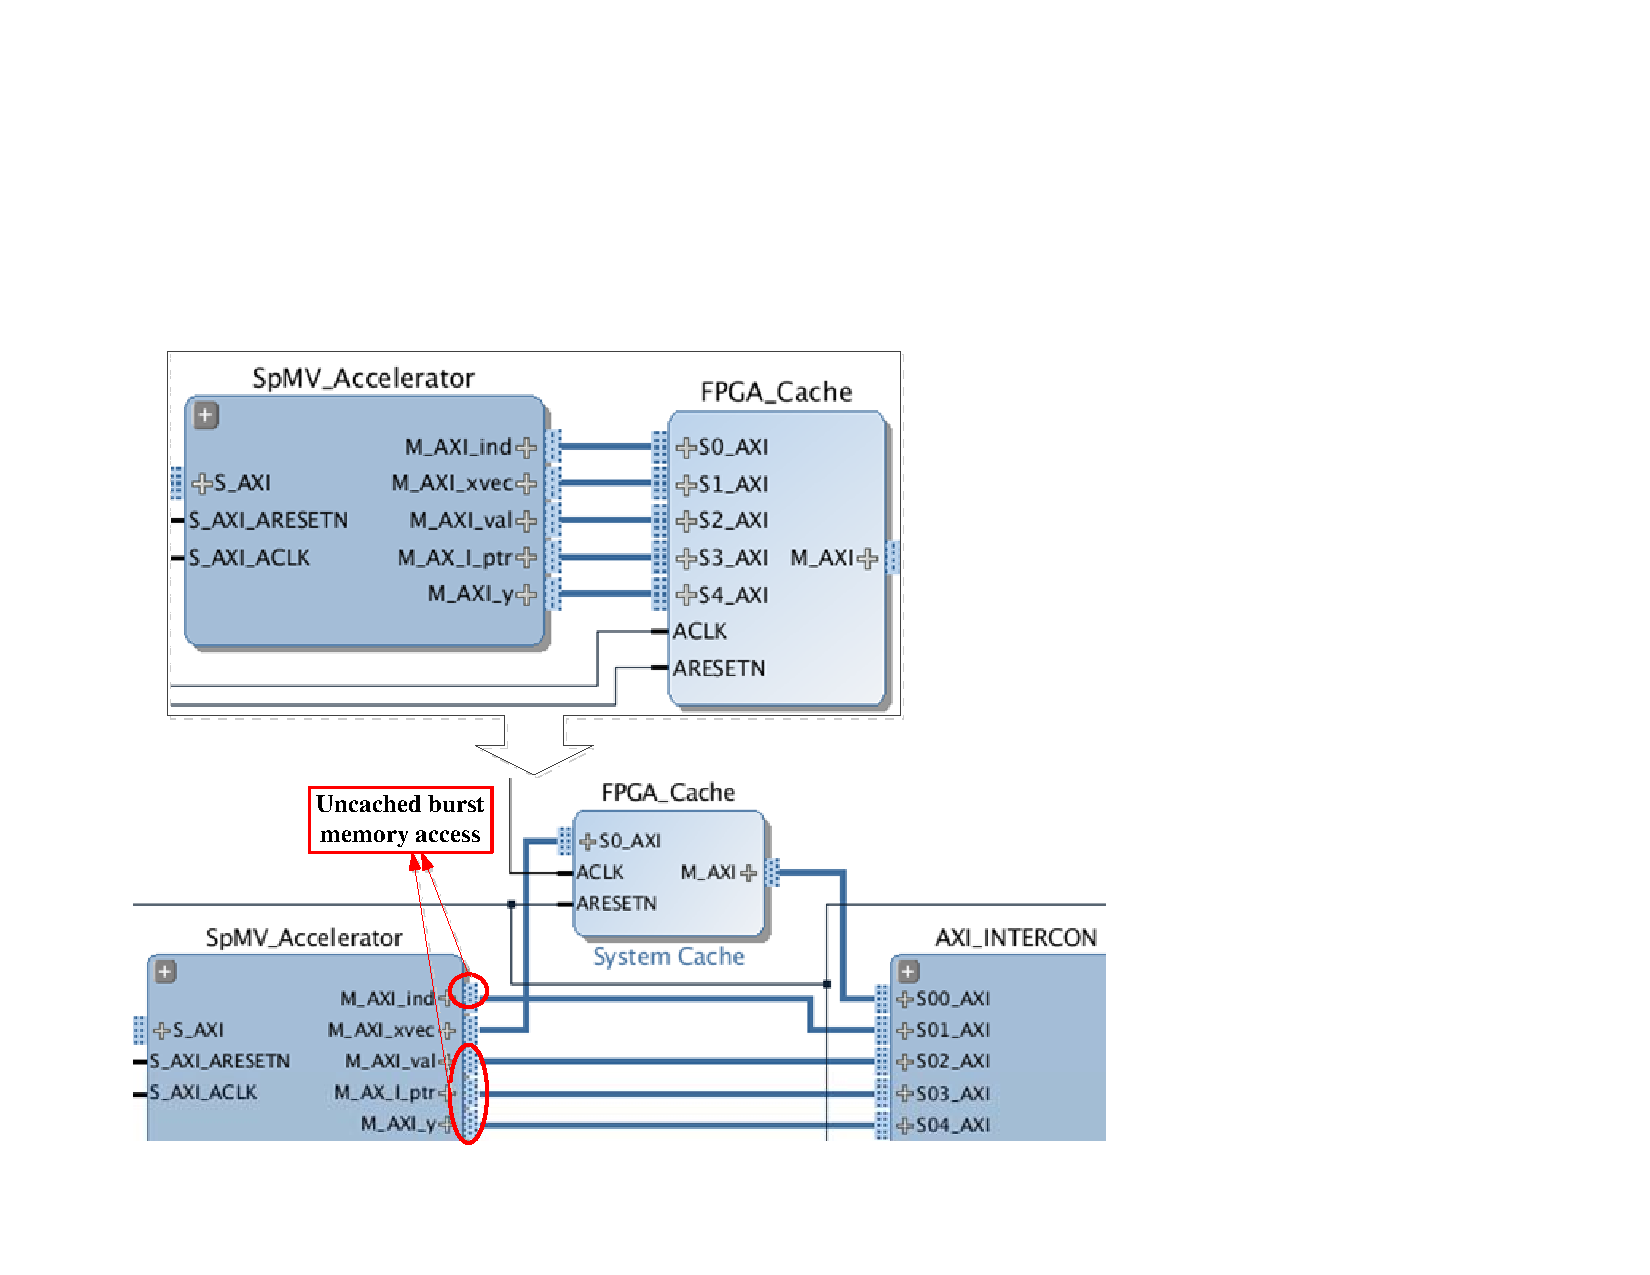
\includegraphics[width=0.65\linewidth]{chap3fig/memOptConv.pdf}
\caption{Optimized Data Access Mechanism
\label{fig:from2}}
\end{center}
\end{figure}
Shown in figure~\ref{fig:from2} is an example where the described techniques are applied to one of our benchmarks.
The cache added between the accelerator and the memory subsystem was originally shared by the five memory
interfaces. However,
as four of those will load/store data in continuous addresses, they can be converted to burst accesses.
The cache is now exclusively used by ``xvec'' which accesses data randomly. The benefits of these transformations
will be quantified in section~\ref{sec:er}.


\section{Hardware Generation}

To create the RTL implementation from each subgraph,
we convert the LLVM intermediate representation back to C
syntax and then feed it to an existing HLS tool. By building a
source to source transformation flow, we can ensure portability
across different back-end RTL generation tools.
At the instruction level, the LLVM to C translation is rather
straightforward. Most LLVM IR instructions can be mapped
directly to C statements, as seen in figure~\ref{fig:totalFlow}. The only nontrivial
transformation we perform is in dealing with the $\phi$ operations, which generate
 values of variables based on the the incoming control edges.  In the case where the source instruction for an operand is within the same subgraph, instead of
 producing to the operand, this source instruction writes directly to the output
 of the $phi$ operator.
 On the other hand, if the source
is in another subgraph, a load operation is inserted to the basic block
where the data is produced, but again assigning the result directly
to the output variable of $\phi$. The $\phi$
instruction itself can be removed. An example of this conversion is
shown in figure~\ref{fig:phi2c}.


\begin{figure}[htp]
\begin{center}
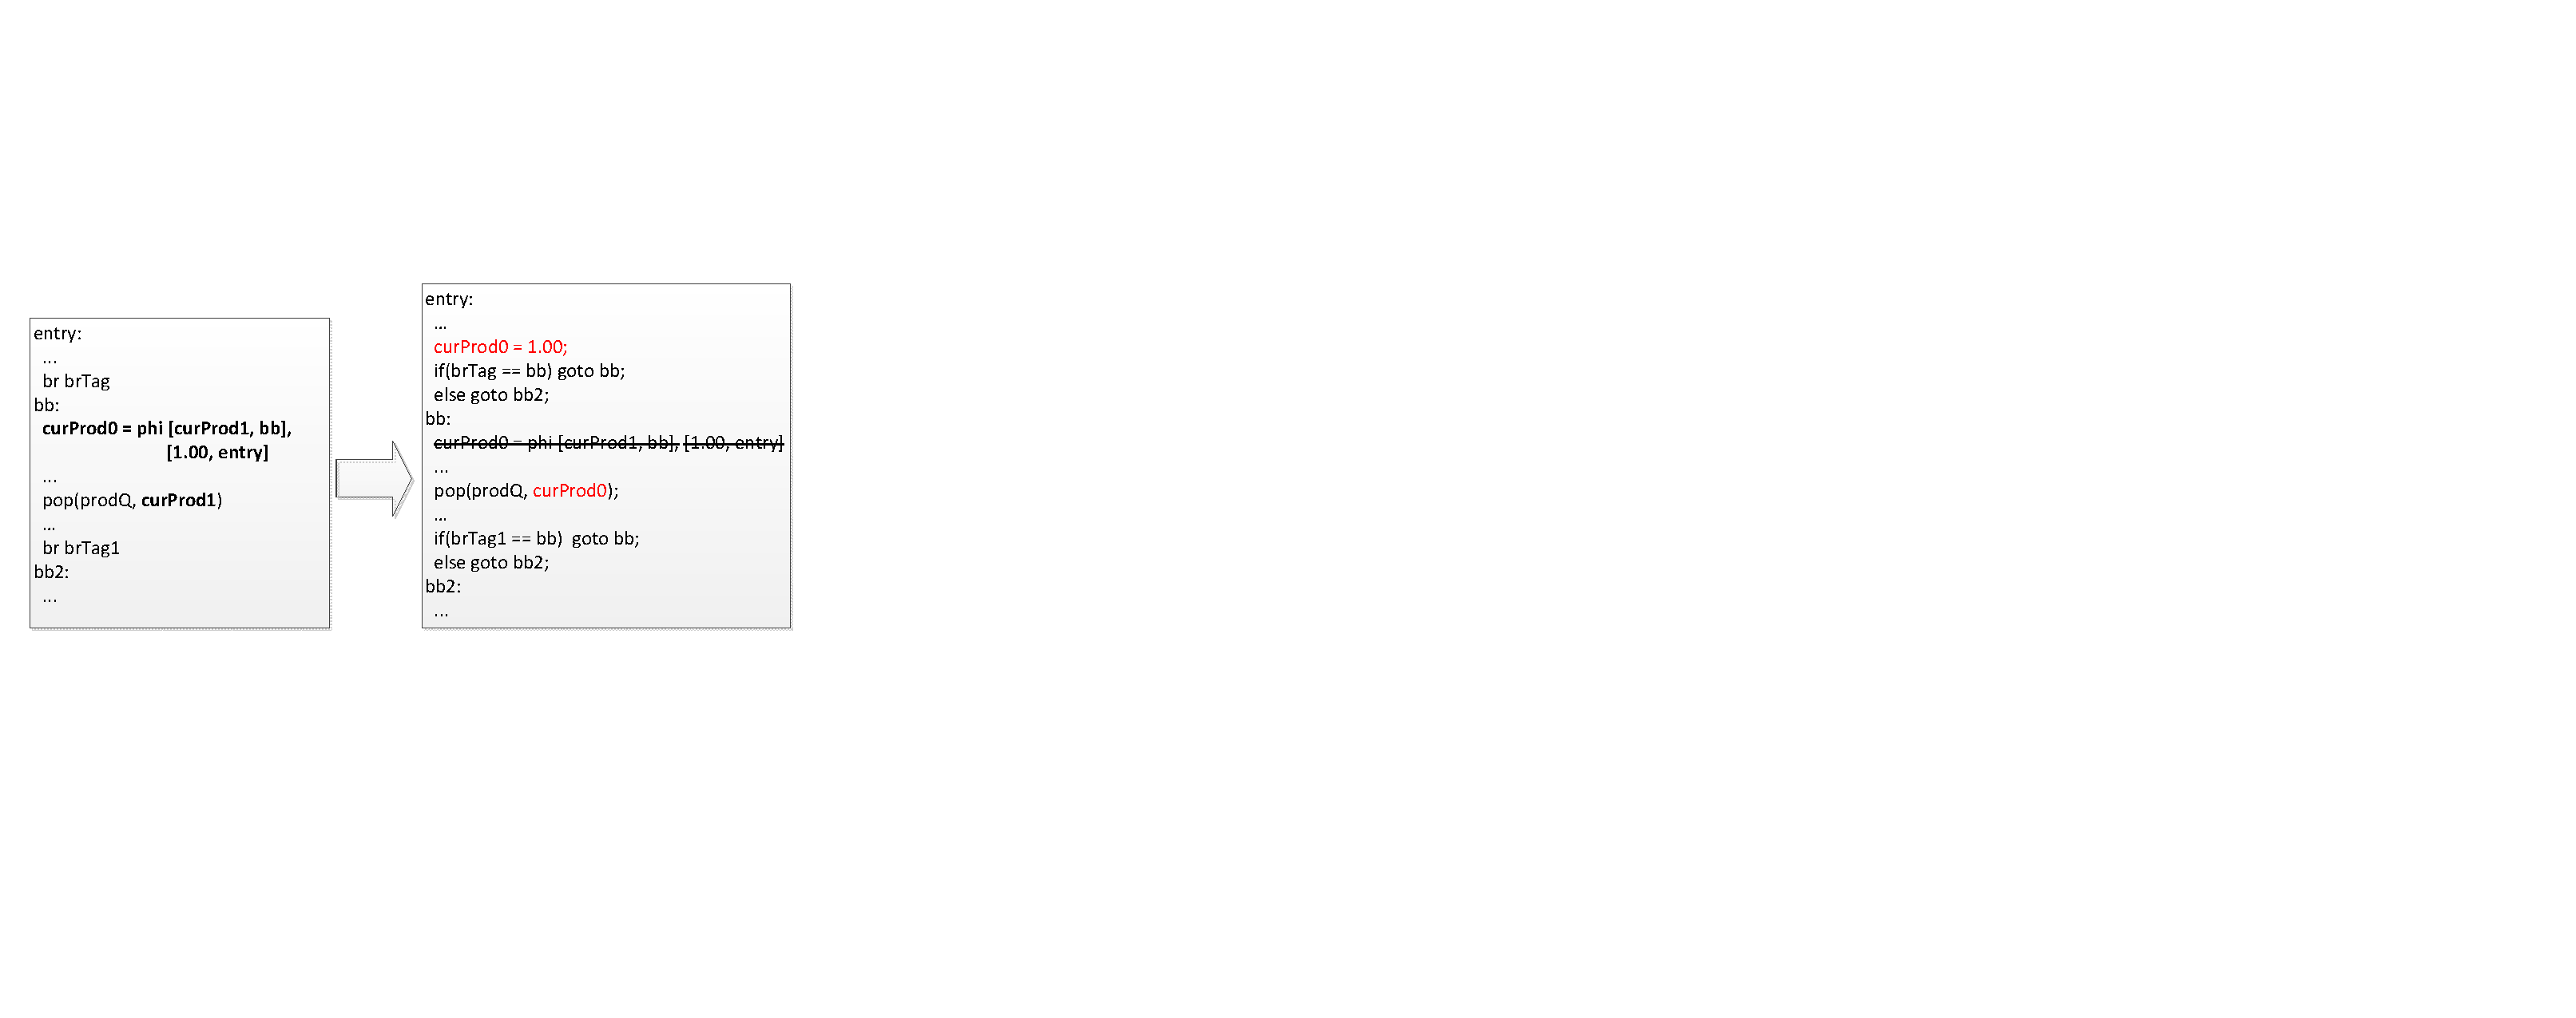
\includegraphics[width=0.7\linewidth]{chap3fig/SSA2C.pdf}
\caption{Converting $\phi$ Operator to C
\label{fig:phi2c}}
\end{center}
\end{figure}
\begin{comment}
As each subgraph contains instructions from only a subset
of the basic blocks in the original program, it does not always
have a complete control flow. To ensure each processing
module generated is self-contained and has well-defined behavior,
extra basic blocks are sometimes added. Our tool finds
the nearest common dominator of all the basic blocks in a
subgraph and add all the control flow statements between this
dominator and the other basic blocks. Consequently, there
is a unique entry block for every subgraph, and different
module will traverse the exact same execution path when the
processing pipeline is active.
\end{comment}

For the next step, where all the components are to be connected
together, we rely on the FIFO generators provided by Xilinx.
Similarly, on-FPGA cache and the
interconnect, which is used to bridge the computational pipeline
and the memory subsystem, are also parametrized Xilinx IPs. 
Within our flow, TCL script is generated according to the communication requirement of the subgraphs. The construction of the whole pipeline
is then performed in Xilinx Vivado IP Integrator by invoking this TCL script.
All the steps involved in our
pipeline generation flow are summarized in figure~\ref{fig:allsteps}.
\begin{figure}[htp]
\begin{center}
\includegraphics[width=0.8\linewidth]{chap3fig/flowSteps.pdf}
\caption{Pipeline Generation Flow
\label{fig:allsteps}}
\end{center}
\end{figure}

%\section{Proof of Liveness}
\section{Experimental Evaluation}
\label{sec:er}
\subsection{Experiment Setup }
To demonstrate the benefits of our approach, processing pipelines
are synthesized and physically implemented on FPGA. The particular device used for the experiments is the Zynq-7000 XC7Z020 FPGA
SoC from Xilinx, installed on the ZedBoard evaluation platform. 
The SoC is divided into two parts: an ARM-processor based processing system (PS), and the programmable logic (PL). 
The baseline 
for our evaluation is the performance of each software kernel running
on the ARM core in the SoC. It is an out of order, dual issue hard
processor running at 667MHz. The Zynq platform also provides two
options for the reconfigurable accelerators to access the main memory subsystem: 
through the accelerator coherence port (ACP), or the high performance (HP) port. 
The former connects to the snoop control unit in the processing system and 
thus uses/modifies the processing system's on chip cache. The HP port connects
directly to the memory controller, which necessitates the flushing of cache lines 
by the processor if a cached data structure is accessed by the accelerator.
In either case, if memory states are also buffered in the reconfigurable array with caches, they 
need to be explicitly pushed to the processing system side after the accelerator finishes running. As both ACP
and HP are slave ports, they provide no mechanisms to extract data from the FPGA
when the ARM processor is running. The interaction between the generated accelerators
and the main pieces of the FPGA SoC is shown in figure~\ref{fig:ippf}.


\begin{figure}[htp]
\begin{center}
\includegraphics[width=0.7\linewidth]{chap3fig/ippf.pdf}
\caption{Implementation of Computational Pipeline in FPGA SoC  
\label{fig:ippf}}
\end{center}
\end{figure} 
In our study, Vivado HLS, a state-of-the-art high level synthesis tool provided by Xilinx,
is used for generating the conventional accelerator (Con.ACC) as well as the individual
modules in our decoupled computational pipeline (DCP). With the target clock period set to 
8ns during HLS, the tightest timing constraints post place \& route implementations managed to meet range from 111 to 150MHz. 
All design points shown in this section 
use the highest achievable frequency as the actual operating clock frequency. 

\subsection{Benchmark Descriptions}
The target application of our flow are algorithms where control flow and
data access patterns depend on run time data or results of computation.
The four irregular kernels listed below are pushed through our flow:
%from several benchmark kernels. These benchmarks
%are non-regular, as their control flow and data access patterns 
%depend on the runtime data. 
\begin{itemize}
    \item \textbf{Sparse matrix vector (SpMV) multiply} is a computation kernel that has been studied, transformed
and benchmarked many different ways in various research projects. Our purpose here is not to produce the best-performing SpMV multiply using special data structure and memory allocation schemes. Rather, we use the most basic and widely used algorithm and storage format to evaluate how much benefit our flow can provide.
The input matrix is stored in
compressed sparse row (CSR) format. 
Loads from
an index array are performed before numbers can be fetched
for the actual floating point multiply. 

\item \textbf{Knapsack } is a problem in combinatorial optimization. Given a collection of
items, each with its own weight and value, knapsack tries to select a subset of them such that the total profit is maximized while the weight limit is not violated.
It is a classic problem which is often solved using dynamic programming, where the memory addresses accessed come from computation.
It is therefore hard to prefetch the needed data unless the entire dataset fits
in on chip buffer.
%only available during run time, and therefore the exact locations where the variable opt_without is loaded from are not known a priori. 

\item \textbf{Floyd-Warshall} takes a graph as input and computes the shortest distances between any pairs of vertices. Similar to knapsack, it is solved by
dynamic programming. Even though all memory references are regular, i.e. simple functions of the loop indices, the control flow depends on the results of computation.

\item \textbf{Iterative depth first search} is again a widely used graph algorithm. The version used for our experiment makes use of a stack and operates on pointer based data structures. 
 
\end{itemize}

The irregularity in
memory accesses and execution paths in these benchmarks makes it hard for existing
HLS tools to directly generate efficient hardware. The conventional accelerators, when
implemented on the FPGA, are also very sensitive to the latency
of data accesses, due to the high ratio of memory operations to computation.

\begin{table}[htbp]
\caption{Input Data Set for the Benchmarks}
\centering
\begin{tabular}{| c | c | c | }
  \hline            
  
 \multirow{2}{*}{Benchmark}   &   \multirow{2}{*}{Description of Input Data} & \multirow{2}{*}{Total Size of Input Data}\\
 &       &   \\
  \hline            
  \hline            
\multirow{2}{*}{}SpMV&  Matrix dimension = 4096 & \multirow{2}{*}{ $\approx$ 16 MB}  \\
%\cline{2-3}                                                                                                                                                    
 Multiply &Density of Matrix = 0.25       &  \\
%\cline{2-3}                                                                                                             
   \hline                                                                                                           
\multirow{2}{*}{Knapsack}&  Weight Limit = 3200 &\multirow{2}{*}{$\approx$ 5 MB}  \\
%\cline{2-3}                                                                                                                                                    
  &Number of Items = 200       &   \\
%\cline{2-3}                                                                                                             
\hline
\multirow{2}{*}{}Floyd-& \multirow{2}{*}{Number of Nodes = 1024}  & \multirow{2}{*}{$\approx$ 8 MB}  \\
%\cline{2-3}                                                                                                                                                    
 Warshall &       &   \\
%\cline{2-3}                                                                                                             
\hline
\multirow{2}{*}{}Depth-First&  Number of Nodes = 4000 & \multirow{2}{*}{$\approx$ 3 MB}  \\
%\cline{2-3}                                                                                                                                                    
 Search & Number of Neighbors per Node = 200       &   \\
%\cline{2-3}                                                                                                       
  \hline                                                                                                           
\end{tabular}
\label{tab:datasize}
\end{table}


Table~\ref{tab:datasize} describes the characteristics of the input data set for each
benchmark. 
As our approach is primarily used for cases where off-chip communication plays a
significant role in determining the final performance, the input data size are chosen
to be much larger than typical on-FPGA cache. For smaller problems where the
entire input data set can be buffered on chip, the conventional DMA+accelerator approach,
as described in~\cite{vivado_hls:appnoteMMult}, would not suffer from variable data access
latency and our decoupled computational pipelines would offer little advantage.




\begin{figure}[htp]
\begin{center}
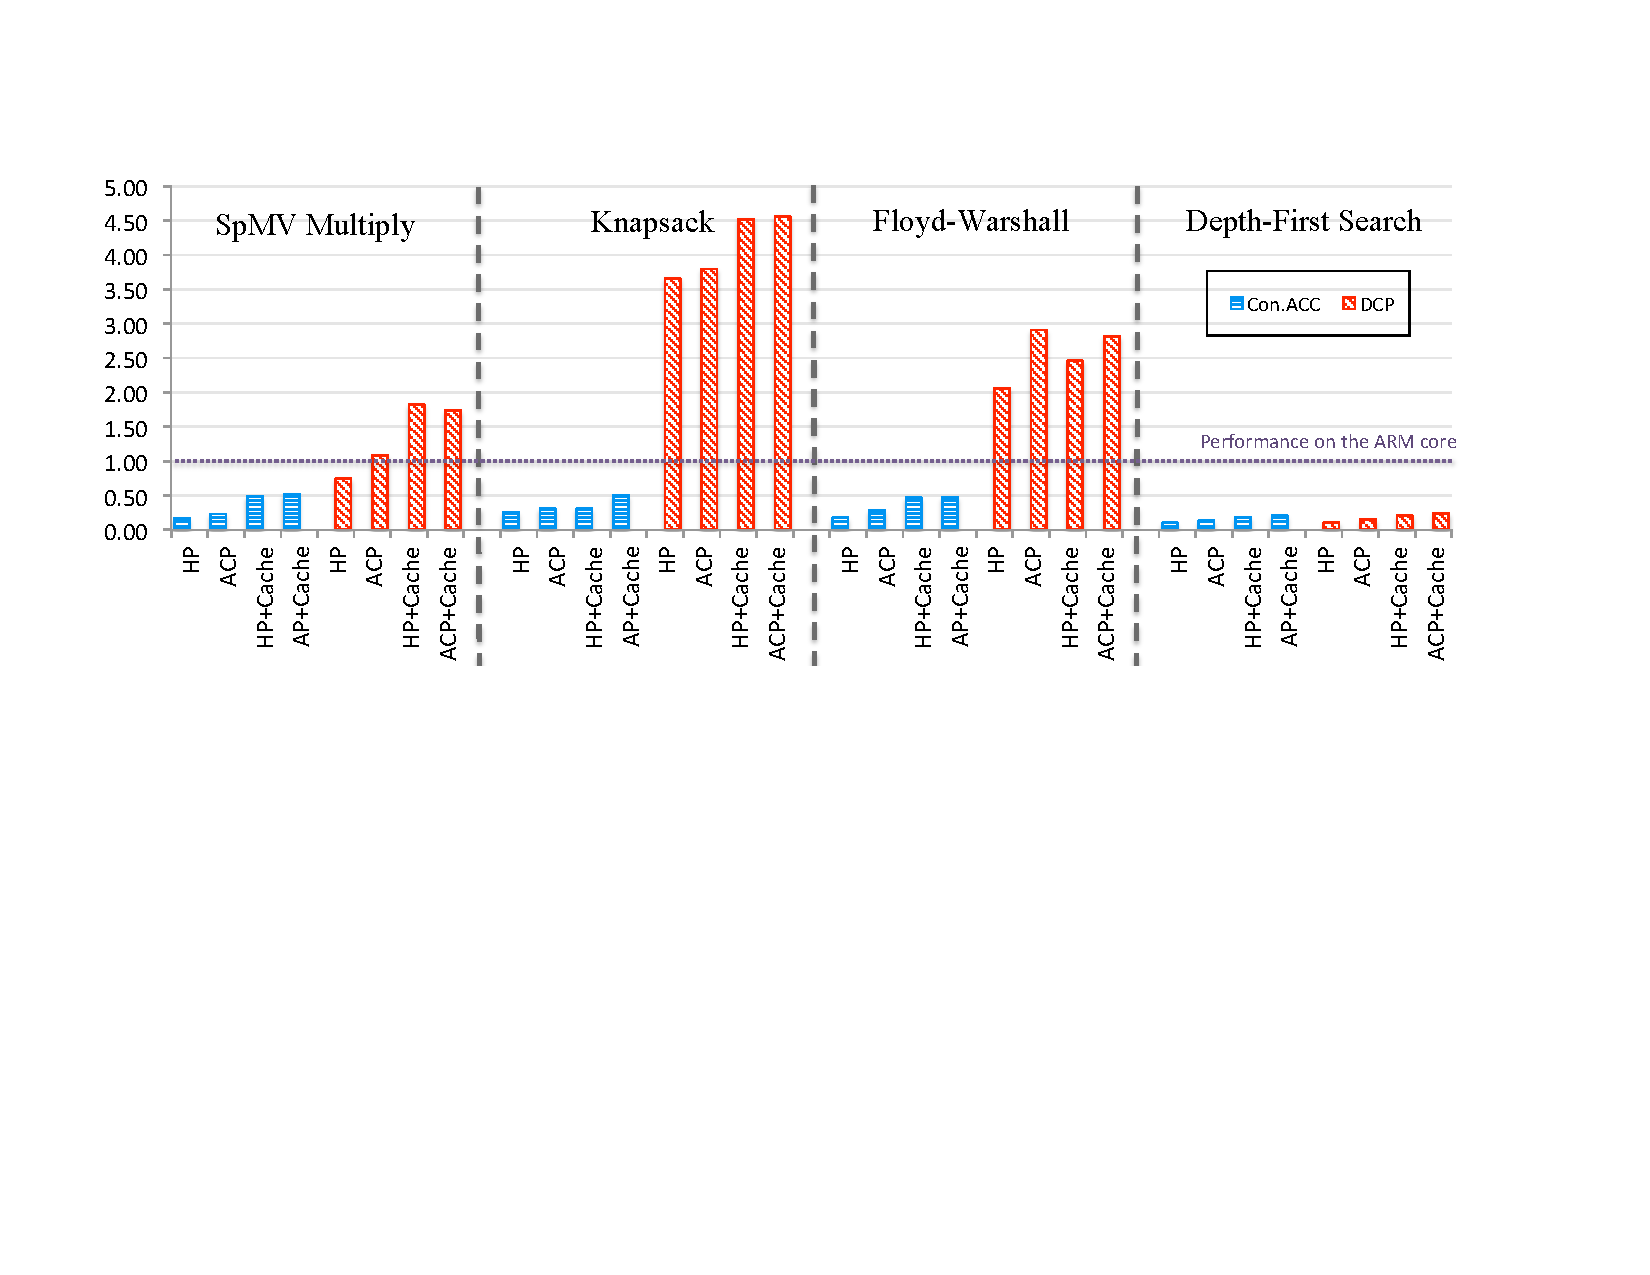
\includegraphics[width=1.0\linewidth]{chap3fig/thesis_perf.pdf}
\caption{Performance of Conventional Accelerators and Decoupled Computational Pipelines
\label{fig:acpraw}}
\end{center}
\end{figure}



\subsection{Performance Comparisons}
\begin{comment}
To provide context for our comparison and highlight the weakness of accelerators generated directly using HLS, we show the performance of a set of conventional accelerators in figure~\ref{}. All the numbers in the figure are normalized to the baseline (software running
on hard ARM core).

These conventional accelerators are supported with different configurations of the memory subsystem. Direct connection to HP port generally incurs the highest memory access latency as
the data are not cached in the PS or the PL. The latency is reduced when ACP is used. To
bring the data even closer to the accelerator, caches can be instantiated on PL. Our implementations use Xilinx system cache IP, configured to be 64KB and 2 way associative.

From this figure, there is a very clear trend that the overall performance increases significantly as the data get cached closer to the accelerators. Across the four benchmarks, the ratio of the fastest to the slowest design points is, on average, 2.4x. The throughput is apparently rather sensitive to the memory access latency. Meanwhile, even the fastest configurations here are slower compared to the baseline. With caches on PL, the conventional accelerators, on average, only achieves throughput about 40\% that of the baseline.
The superscalar, out-of-order ARM core is capable of exploiting instruction level parallelism to a good extent and also has a high performance on-chip cache.
The additional parallelism extracted by the HLS tool is evidently not enough
to compensate for the clock frequency advantage the hard processor core has over the programmable logic and the longer data access latency from the reconfigurable array. 


Now we look at the performance of the decoupled computational pipelines (figure~\ref{}).
Similar to the conventional accelerators, these pipeline's throughput also increase
as the data latency reduces. However, the differences between the different memory subsystem
configurations are significantly smaller. The fastest configuration is only 1.7x better than 
the slowest, which demonstrate how the effect of data access latency is reduced in our
generated pipelines. Also, compared to the baseline, the DCPs provide much better performance.
On average, the 

To highlight the difference in raw performance, the fastest conventional accelerators and the decoupled computational pipelines are compared side by side in figure~\ref{}. There is a very
clear performance advantage



To understand the pros and cons of different optimization options and support infrastructure configurations, we have generated an array of different design points for each benchmark.
Every design point represents a different trade off between performance and area cost. 

\subsubsection{Sparse Matrix Vector Multiply}
Sparse matrix vector (SpMV) multiply is a computation kernel that has been studied, transformed
and benchmarked many different ways in various research projects. Our purpose here is not to produce the best-performing SpMV multiply using special data structure and memory allocation schemes. Rather, we want to see, given the most basic and widely used algorithm description, how
much benefit our flow can provide.

To provide 

We want to examine how the partitioning of operations and the subsequent optimization affect the performance and area. Here we connect a few different instances of the DCPs generated to the HP port of the processing system, and compare them against the directly generated Con.ACCs.


Figure~\ref{}, shows the performance and area of a few design points
\end{comment}

In figure~\ref{fig:acpraw}, performance of the conventional accelerators and decoupled computational pipelines are compared, all the numbers are normalized to the baseline.
Both Con.ACC and DCPs are supported with different memory subsystem configurations.
%Conventional accelerators and decoupled computational pipelines with different memory subsystem
%configurations are compared.  
Direct connections to the HP port generally incur the highest memory access latency as
the data are not cached in the PS or the PL. This latency is reduced when ACP is used. To
bring the data even closer to the accelerator, cache IPs can be instantiated on the PL. Our implementations use Xilinx's system cache IP, configured to be 64KB and 2 way associative.


In all four benchmarks, accelerators generated directly from software kernels using conventional HLS flow
actually result in a performance degradation compare to running the kernels on the hard processor. The fastest Con.ACC implementations with
on-PL caches, only manage to achieve throughput less than 50\% that of the baseline. 
The superscalar, 
out-of-order ARM core is capable of exploiting instruction level parallelism to a good extent 
and also has a high performance on-chip cache.
The additional parallelism extracted by the HLS tool is evidently not enough
to compensate for the clock frequency advantage the hard processor core has over the programmable logic and the longer data access
latency from the reconfigurable array. 

With our methodology, the computational pipelines generated 
are rather competitive against the hard processor, even
without a reconfigurable cache. For SpMV multiply, knapsack and Floyd-Warshall, when DCPs are directly connected to the PS through the ACP, 
the average performance is 2.3 x that of the baseline---representing
an 8.4 x gain over the conventional accelerators.
Upon the addition of on-PL caches,  
the average runtime of DCPs was further reduced by 18.7\%, making the DCPs about 2.9x faster than the baseline.

It is also apparent that our approach has its limitations, as demonstrated by its ineffectiveness in the benchmark depth first search.
The kernel performs very little computing but lots of memory accesses.
The use of a stack in DFS also creates a dependence cycle through the memory
and consequently, the performance is fundamentally limited by the latency of memory access.
Thus there were only small differences between the performance of the conventional accelerator and the decoupled computational pipeline. Besides, the memory access pattern
does not provide many opportunities for optimizations. As a result, DCP and Con.ACC achieves performance far below that of the baseline, 
which has a much higher clock frequency and a faster cache.     


The figure also allows us to examine the effect of different memory configurations on the overall performance of the design. There is a general trend that the performance improves as the 
data get cached closer to the computation engine. For conventional accelerators, the ratio of the fastest to the slowest design points is, on average, 2.4x. For decoupled computational pipeline,
this ratio is reduced to 1.7x. The relative insensitivity of the DCPs towards data access latency
is rather evident from this difference.
\begin{comment}
The throughput is apparently rather sensitive to the memory access latency.

while that of the conventional
accelerators was cut by 45.4\%. The gap between their performance is thereby reduced from 8.4 to 5.6 times. 
%This difference is due to conventional accelerators' sensitivity to the latency of data accesses, which
%is also manifested by its performance degradation of 40\% when the uncached HP port is used instead of ACP. 
\end{comment}

Overall, for kernels suitable for FPGA acceleration, there is a significant performance advantage in using
decoupled computational pipelines. If we compare the best results using DCP to conventional accelerators, we see improvement
of 3.3 to 9.1 times, with an average of 5.6. 

\begin{table}[htbp]
\caption{Resource Usage of Accelerators.}
\centering
\begin{tabular}{| c | c | c | c | c | c | c | c| }
  \hline            
  \multirow{2}{*}{} &  &   \multicolumn{3}{c|}{ACP  } & \multicolumn{3}{c|}{ ACP + 64KB Cache }   \\
 \cline{3-8} 
 {Benchmark}   &    & LUT& FFs& BRAM & LUT &	 FFs    	& BRAM    \\
  %
  %                 & LUT &FFs&  BRAM &  LUT &	 FFs    	& BRAM   \\
  \hline            
  \hline            
\multirow{3}{*}{}&Con.ACC  & 9873 &9116 &10 & 7918 & 6792 & 21  \\
\cline{2-8}                                                                                                                                                    
SpMV &DCP       & 8577 & 8837& 10 & 6718  &6788 & 21\\
\cline{2-8}                                                                                                             
    Multiply   &\% change & -13.1 &-3.1 & 0 & -15.2  & -0.1 & 0  \\
  \hline                                                                                                           
\multirow{3}{*}{}&Con.ACC  & 7672 &7490 &8 & 6573 & 5885 & 21  \\
\cline{2-8}                                                                                                                                                    
Knapsack &DCP       & 8089 & 8787& 8 & 6970  &7256 & 21\\
\cline{2-8}                                                                                                             
       &\% change & +5.4 &+17.3 & 0 & +6.0  & +23.3 & 0  \\
  \hline                                                                                                           
\multirow{3}{*}{}&Con.ACC  & 2491 &3528 &0 &3806  &4629  &19   \\
\cline{2-8}                                                                                                                                                    
Floyd- &DCP       & 7659 &7210 &0  &8995  &8309 &19 \\
\cline{2-8}                                                                                                             
 Warshall      &\% change &+207.5  &+104.3 & 0 & +104.4  & +79.5  & 0  \\
  \hline                                                                                                           
\multirow{3}{*}{}&Con.ACC  & 4810 &4929 &4 & 4931 & 4594 & 21  \\
\cline{2-8}                                                                                                                                                    
DFS &DCP       & 8509 & 7813& 4 & 7436  &6298 & 21\\
\cline{2-8}                                                                                                             
       &\% change & +76.9 &+58.5 & 0 & +50.8  & +37.1 & 0  \\
  \hline                                                                                                           

\end{tabular}
\label{tab:areacom}
\end{table}







\subsection{Area comparison}
To quantify the impact of our proposed methodology on area, 
we have compared the FPGA resouce usage of conventional accelerators and
the decoupled computational pipelines.
Table~\ref{tab:areacom} shows the results, 
where each acclerator is complemented with two different memory subsystem configurations.

The difference in area between DCPs and Con.ACCs is effected by
two factors.  There are additional costs associated with the communication primitives 
and FIFOs for the DCP implementations. 
On the other hand,   
the original programs are partitioned into subgraphs and separately turned into hardware
in DCPs, which sometimes can reduce the depth of the internal 
pipeline in the processing modules, resulting in area savings. 
%as compared to the instantiation
%of the same set of operators in conventional accelerators. 
%For instance,
%in our motivating example, the initiation interval of the inner loop is 
%determined by the floating point multiply. The loop counter, which is
%another SCC in our dataflow, will also need
%to be synchronized to the same schedule, which necessitate insertion of
%additional pipeline stages. 
The overall change therefore depends on which factor plays a larger role, and is 
ultimately application specific. 


\section{Discussion}
The experimental results have validated the general approach we have proposed and implemented. 
Decoupling of execution between different part of the control dataflow graph can yield
significant benefits. How the graph should be split however, is a space worth exploring.

The algorithm we have devised is simplistic and easy to implement.
It is also very aggressive in that all separable memory accesses are assigned to a new partition.
Furthermore, as we perform topological sort on the nodes before partitioning them, many
edges might be cut when a new subgraph is created, especially when the dependencies between instructions are relatively denser.
Therefore, as the input kernels increase in size, our algorithm may result in pipelines with prohibitively high number of communication channels. The optimization we described in section~\ref{dupvscomm}
partially addresses this issue, but it does not reduce the total number of subgraphs.


\begin{comment}
To alleviate this particular issue, we can make the whole pipeline generation process more
flexible. While the instruction partitioning step can be changed and various techniques can be
experimented with, the construction of executable subgraphs and the synthesis of hardware
are invariant across different partitioning schemes. Optimizations like pipelining of memory
requests can still be applied if it can be accommodated by the structure of the reconstructed
subgraphs. Within this context, several possible partitioning heuristics may be worth trying out
in the future.

The algorithm we have implemented ensures the data tokens always flow forward, as the
partitioning is performed on a directed acyclic graph. The benefit si
\end{comment}